\documentclass[12pt,fleqn]{article}\usepackage{../../common}
\begin{document}
Materyel Mekaniği - 6

Dönüş (Rotation)

Alttaki gibi bir kiriş düşünelim,

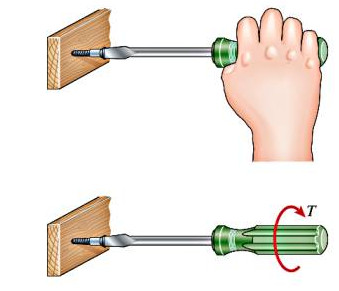
\includegraphics[width=20em]{phy_020_strs_06_01.jpg}

Daha önce bu tür bir kiriş üzerinde eksenel yöndeki kuvvetler ve yer
değişimlerinin ilişkisini

$$
\left[\begin{array}{c}
f'_{1x} \\ f'_{2x}
\end{array}\right] =
\frac{AE}{L}
\left[\begin{array}{cc}
1 & -1 \\ -1 & 1
\end{array}\right]
\left[\begin{array}{c}
u'_1 \\ u'_2
\end{array}\right]
\mlabel{1}
$$

olarak göstermiştik. Üstte yazılan kirişin yerel, kendisine has kordinat
sistemini baz alıyor. Eğer üstteki değişkenleri global kordinat sistemine
eşlemek, yansıtmak istiyorsak o zaman sistemi görülen $\theta$ kadar döndürmemiz
gerekiyor. Döndürme işlemi genel olarak iki boyuttaki bir $[u, v]$ vektörü için
[1, sf. 85]

$$
\left[\begin{array}{c}
u' \\ v'
\end{array}\right] =
\left[\begin{array}{cc}
C & S \\ -S & C
\end{array}\right]
\left[\begin{array}{c}
u \\ v
\end{array}\right]
\mlabel{2}
$$

ile yapılır, ki $C = \cos\theta$, $S = \sin\theta$.

Fakat unutmayalım tek eksenlikten çıktığımız zaman kirişin her ucunda iki
serbestlik derecesi vardır, her uç $u,v$ yönünde yer değişim yaşayabilir,
bunları $u_1,v_1$ ve $u_2,v_2$ diye gösterebiliriz. O zaman dönüş hesabı

$$
\left[\begin{array}{c}
u'_1 \\ v'_1 \\ u'_2 \\ v'_2
\end{array}\right] =
\left[\begin{array}{cccc}
C & S & 0 & 0 \\
-S & C & 0 & 0 \\
0 & 0 & C & S \\
0 & 0 & -S & C 
\end{array}\right]
\left[\begin{array}{c}
u_1 \\ v_1 \\ u_2 \\ v_2
\end{array}\right]
$$

İlerlemeden önce iki üstteki dönüş matrisi, $T$ diyelim, hakkında ilginç bir
ispatı verelim, ileride lazım olacak. Acaba $T^T = T^{-1}$ ifadesi doğru mudur?
Bu aynı zamanda [1] kitabındaki 3.28 probleminin de cevabı. İspat için $T T^T$
çarpımını yapabiliriz, eğer birim (identity) matrisi elde edersek ispat tamam
demektir.

$$
T = 
\left[\begin{array}{cccc}
C & S & 0 & 0 \\
-S & C & 0 & 0 \\
0 & 0 & C & S \\
0 & 0 & -S & C 
\end{array}\right], \quad
T^T = 
\left[\begin{array}{cccc}
C & -S & 0 & 0 \\
S & C & 0 & 0 \\
0 & 0 & C & -S \\
0 & 0 & S & C 
\end{array}\right]
$$

Çarpımı \verb!sympy! ile yapalım,

\begin{minted}[fontsize=\footnotesize]{python}
from sympy import symbols, pprint, latex
from sympy.matrices import Matrix
C,S = symbols("C,S")
T = Matrix([[C,S,0,0],[-S,C,0,0],[0,0,C,S],[0,0,-S,C]])
Tprime = Matrix([[C,-S,0,0],[S,C,0,0],[0,0,C,-S],[0,0,S,C]])
print (latex(T * Tprime)[:60],'...')
\end{minted}

\begin{verbatim}
\left[\begin{matrix}C^{2} + S^{2} & 0 & 0 & 0\\0 & C^{2} + S ...
\end{verbatim}

\LaTeX\ ile

$$
\left[\begin{matrix}C^{2} + S^{2} & 0 & 0 & 0\\0 & C^{2} + S^{2} & 0 & 0\\0 & 0 & C^{2} + S^{2} & 0\\0 & 0 & 0 & C^{2} + S^{2}\end{matrix}\right]
$$

Hatırlarsak $C = \cos\theta, S = \sin\theta$, bunları yerine koyunca tüm köşegen
boyunca 1 değeri elde edilir, diğer hücrelerde sıfır var, demek ki bir birim
matrisi elde ettik. Bu demektir ki $T T^T = I$, ve bu ifadenin doğru olmasının
tek yolu $T^T = T^{-1}$ olmasıdır.

Bir önemli eşitlik daha, hem yer değişimleri, hem kuvvetler döndürme
matematiğini kullanabilirler. Mesela dönüş matrisi $T$ için

$$
d' = T d
$$

diyebilirdim, ya da kuvvetler için

$$
f' = T f
$$

Bunun bir yan etkisi şudur, yer değişimlerini kuvvetlerle ilintilendiren
sistem

$$
f = k d
$$

ise,

$$
f' = k' d' 
$$

sistem şöyle de gösterilebilir,

$$
T f = k' T d
$$

Eğer üstteki ifadeyi soldan $T^{-1}$ ile çarparsak,

$$
T^{-1} T f = T^{-1} k' T d
$$

$T^{-1} T = I$ olduğu için yokolur, ayrıca biraz önceki ispattan $T^{-1} = T^T$
olduğunu biliyoruz,

$$
f = T^T k' T d
$$

Global direngenlik matrisi $k$ ortadaki $T^T k' T$ büyüklüğüdür.

Devam edelim. Dönüş mekaniğini gördük, şimdi önceki derste işlenen kiriş
parçasına hem eksenel dinamiği hem de biraz önce gördüğümüz dönüş mantığını
ekleyelim.  Altta görülen kiriş parçasının hareketlerini hesaplayabilmek
istiyoruz yani,

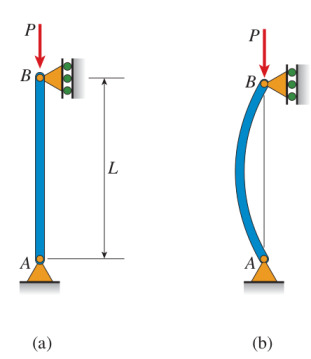
\includegraphics[width=15em]{phy_020_strs_06_02.jpg}

Önceki dersten hatırlarsak eksene dik yük alan parçaların mekaniği alttaki
formülle gösterilmişti,

$$
\left[\begin{array}{c}
f_{1y} \\ m_1 \\ f_{2y} \\ m_2
\end{array}\right] =
\frac{EI}{L^3}
\left[\begin{array}{cccc}
12 & 6L & -12 & 6L \\
6L & 4L^2 & -6L & -6L \\
-12 & -6L & 12 & -6L \\
6L & 2L^2 & -6L & 4L^2
\end{array}\right]
\left[\begin{array}{ccc}
v_1 \\ \phi_1 \\ v_2 \\ \phi_2
\end{array}\right]
$$

Bu formüle (1)'deki eksenel mantığı eklersek, yerel kordinatlarda

$$
\left[\begin{array}{c}
f'_{1x} \\ f'_{1y} \\ m'_1 \\ f'_{2x} \\ f'_{2y} \\ m'_2
\end{array}\right] =
\left[\begin{array}{cccccc}
C_1 & 0 & 0 & -C_1 & 0 & 0 \\
0 & 12C_2 & 6 C_2 L & 0 & -12 C_2 & 6 C_2 L \\
0 & 6C_2 L & 4 C_2 L^2 & 0 & -6 C_2 L & 2 C_2 L^2 \\
-C_1 & 0 & 0 & C_1 & 0 & 0 \\
0 & -12C_2 & -6 C_2 L & 0 & 12 C_2 & -6 C_2 L \\
0 & 6 C_2 L & 2 C_2 L^2 & 0 & -6C_2 L & 4C_2 L^2
\end{array}\right]
\left[\begin{array}{c}
u'_1 \\ v'_1 \\ \phi'_1 \\ u'_2 \\ v'_2 \\ \phi'_2
\end{array}\right]
$$

elde edilir, ki $C_1 = \dfrac{AE}{L}$ ve $C_2 = \dfrac{EI}{L^3}$
olmak üzere. Üstte ortada duran matris $k'$ matrisidir.

Şimdi dönüş mekaniğini ekleyelim.

$$
\left[\begin{array}{ccc}
u'_1 \\ v'_1 \\ \phi'_1 \\ u'_2 \\ v'_2 \\ \phi'_2 
\end{array}\right] =
\left[\begin{array}{cccccc}
C & S & 0 & 0 & 0 & 0 \\
-S & C & 0 & 0 & 0 & 0 \\
0 & 0 & 1 & 0 & 0 & 0 \\
0 & 0 & 0 & C & S & 0 \\
0 & 0 & 0 & -S & C & 0 \\
0 & 0 & 0 & 0 & 0 & 1
\end{array}\right]
\left[\begin{array}{ccc}
u_1 \\ v_1 \\ \phi_1 \\ u_2 \\ v_2 \\ \phi_2 
\end{array}\right]
$$

Dikkat edersek dönüşümü sağlayan 2 x 2 boyutundaki altmatris, üstteki matristeki
o iki bölge, daha büyük matriste öyle yerleştirildi ki sadece $u_1,v_1$ ve
$u_2,v_2$ değişkenlerini etkiliyor, onlara tekabül eden bölgelerde duruyor.

Böylece $T$ matrisini bulmuş olduk. Şimdi $k$ matrisini hesaplamak için
$k = T^T k' T$ işlemini yapabiliriz [1, sf. 243].

\begin{minted}[fontsize=\footnotesize]{python}
from sympy import symbols, latex, simplify
from sympy.matrices import Matrix
import pickle

C,S,C1,C2,L,A,E,I = symbols("C,S,C1,C2,L,A,E,I")
kprime = Matrix([ [C1, 0, 0, -C1, 0, 0],
                  [0, 12*C2, 6*C2*L, 0, -12*C2, 6*C2*L],
                  [0, 6*C2*L, 4*C2*L**2, 0, -6*C2*L, 2*C2*L**2],
                  [-C1, 0, 0, C1, 0, 0],
                  [0, -12*C2, -6*C2*L, 0, 12*C2, -6*C2*L],
                  [0, 6*C2*L, 2*C2*L**2, 0, -6*C2*L, 4*C2*L**2]])

T = Matrix([[C,S,0,0,0,0],[-S,C,0,0,0,0],[0,0,1,0,0,0],
            [0,0,0,C,S,0],[0,0,0,-S,C,0],[0,0,0,0,0,1]])

res = T.transpose()*kprime*T
res = res.subs(C1,A*E/L) 
res = res.subs(C2,E*I/L**3)
pickle.dump(res,open("frame.pkl","wb")) # sonra lazim olacak diske kaydet
res = res / (E/L) 
print (latex(simplify(res))[:70],'...')
\end{minted}

\begin{verbatim}
\left[\begin{matrix}A C^{2} + \frac{12 I S^{2}}{L^{2}} & \frac{C S \le ...
\end{verbatim}

$$
k = 
\frac{E}{L} \times 
\left[\begin{matrix}A C^{2} + \frac{12 I S^{2}}{L^{2}} & \frac{C S \left(A L^{2} - 12 I\right)}{L^{2}} & - \frac{6 I S}{L} & - A C^{2} - \frac{12 I S^{2}}{L^{2}} & \frac{C S \left(- A L^{2} + 12 I\right)}{L^{2}} & - \frac{6 I S}{L}\\\frac{C S \left(A L^{2} - 12 I\right)}{L^{2}} & A S^{2} + \frac{12 C^{2} I}{L^{2}} & \frac{6 C I}{L} & \frac{C S \left(- A L^{2} + 12 I\right)}{L^{2}} & - A S^{2} - \frac{12 C^{2} I}{L^{2}} & \frac{6 C I}{L}\\- \frac{6 I S}{L} & \frac{6 C I}{L} & 4 I & \frac{6 I S}{L} & - \frac{6 C I}{L} & 2 I\\- A C^{2} - \frac{12 I S^{2}}{L^{2}} & \frac{C S \left(- A L^{2} + 12 I\right)}{L^{2}} & \frac{6 I S}{L} & A C^{2} + \frac{12 I S^{2}}{L^{2}} & \frac{C S \left(A L^{2} - 12 I\right)}{L^{2}} & \frac{6 I S}{L}\\\frac{C S \left(- A L^{2} + 12 I\right)}{L^{2}} & - A S^{2} - \frac{12 C^{2} I}{L^{2}} & - \frac{6 C I}{L} & \frac{C S \left(A L^{2} - 12 I\right)}{L^{2}} & A S^{2} + \frac{12 C^{2} I}{L^{2}} & - \frac{6 C I}{L}\\- \frac{6 I S}{L} & \frac{6 C I}{L} & 2 I & \frac{6 I S}{L} & - \frac{6 C I}{L} & 4 I\end{matrix}\right]
\mlabel{3}
$$

Bu sonuç [1]'deki sonuca benziyor, cebirsel olarak eşit.

Not: $E/L$ bölümünü \verb!sympy! basitleştirmesi öncesi sistemde dışarıdan
uyguladık çünkü cebirsel düzenlemede sisteme yardım etmek istedik, bu sayede
sonuç kitaptaki çıktıya benzemiş oldu.

Cebirsel işlem sonucunu diske kaydettik (3) çıktısı alttaki problemde
lazım olacak. 

Üstteki formül / matris düz katı şasi / düz oynamaz çerçeve (rigid plane frame)
formülü olarak bilinir, bu sistem ``katı bir şekilde birbirine bağlanmış bir
grup kiriş parçalarının toplamı'' olarak ta tarif edilebilir, yani kiriş
parçalarının birbirine olan açıları, yük uygulandıktan sonra bağlandıklarında ne
ise o halde kalırlar, deformasyon sonrası değişime uğramazlar. Ayrıca bu tür bir
sistemde moment bir parçadan diğerine, bağlantı noktaları üzerinden transfer
olabilir, yani katı bağlantı noktaları üzerinden bir moment sürekliliği vardır.

Soru

İlk katı düzlem çerçeve analizi olarak alttaki basit sistemi çözün.

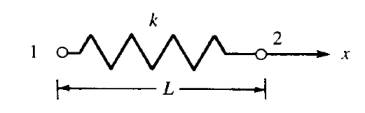
\includegraphics[width=15em]{phy_020_strs_06_03.jpg}

Cevap

Sistem düğüm 1 ve 4 üzerinden sabitlenmiş, düğüm 2 üzerinde ve yatay 40 kN
kuvvet uygulanıyor, ayrıca düğüm 3'te pozitif moment 500 N-m var. Üstteki
resimde global kordinat sisteminin yeri gösteriliyor [1, sf. 244].

Çözüm için her parçayı kiriş matematiği (3) ile formülize edeceğiz, ve bu
parçaları üstdüşüm ile biraraya koyacağız, nihai matrisi çözerek yükleri ve yer
değişimleri bulacağız.

Parça 1

Hesap yapabilmek için (3)'teki matrise ihtiyaç var, bu matrisin sembolik
halini diskten okuyalım, oraya kaydetmiştik, 

\begin{minted}[fontsize=\footnotesize]{python}
from sympy import symbols, latex, simplify
from sympy.matrices import Matrix
import pickle, pandas as pd
pd.set_option('display.max_columns', None)
pd.set_option("display.precision", 4)
C,S,L,A,E,I = symbols("C,S,L,A,E,I")
frame = pickle.load(open('frame.pkl','rb'))
\end{minted}

Birinci parçanın duruş açısı 90 derece, o zaman $C = \cos 90 = 0$, $S = \sin 90 = 1$.
Bu değerleri sembolik matrisi sayısal halee çevirmek için kullanacağız,
\verb!subs! çağrısı ile,

\begin{minted}[fontsize=\footnotesize]{python}
d = {L:3000.0, C:0.0, S:1.0, E:200.0*1e3, A:6500.0, I:80.0*1e6}
res = frame.subs(d) / (1e3*d[E]/d[L])
df1 = pd.DataFrame(np.array(res).astype(np.float64))
df1.columns = ['u1','v1','phi1','u2','v2','phi2']
df1 = df1.round(2)
print ('66.67*1000 * \n', df1)
\end{minted}

\begin{verbatim}
66.67*1000 * 
        u1   v1      phi1      u2   v2      phi2
0    0.11  0.0    -160.0   -0.11  0.0    -160.0
1    0.00  6.5       0.0    0.00 -6.5       0.0
2 -160.00  0.0  320000.0  160.00  0.0  160000.0
3   -0.11  0.0     160.0    0.11  0.0     160.0
4    0.00 -6.5       0.0    0.00  6.5       0.0
5 -160.00  0.0  160000.0  160.00  0.0  320000.0
\end{verbatim}

Matrisin birimi N/mm. 

Parça 2

Bu parçanın duruşu sebebiyle açı sıfır, yani $C=1,S=0$.

\begin{minted}[fontsize=\footnotesize]{python}
d = {L:3000.0, C:1.0, S:0.0, E:200.0*1e3, A:6500.0, I:40.0*1e6}
res = frame.subs(d) / (1e3*d[E]/d[L])
df2 = pd.DataFrame(np.array(res).astype(np.float64))
df2.columns = ['u2','v2','phi2','u3','v3','phi3']
print ('66.67*1000 * \n', df2)
\end{minted}

\begin{verbatim}
66.67*1000 * 
     u2       v2      phi2   u3       v3      phi3
0  6.5   0.0000       0.0 -6.5   0.0000       0.0
1  0.0   0.0533      80.0  0.0  -0.0533      80.0
2  0.0  80.0000  160000.0  0.0 -80.0000   80000.0
3 -6.5   0.0000       0.0  6.5   0.0000       0.0
4  0.0  -0.0533     -80.0  0.0   0.0533     -80.0
5  0.0  80.0000   80000.0  0.0 -80.0000  160000.0
\end{verbatim}

Parça 3

Açı 270 derece, demek ki $C=0,S=-1$.

\begin{minted}[fontsize=\footnotesize]{python}
d = {L:3000.0, C:0.0, S:-1, E:200.0*1e3, A:6500.0, I:80.0*1e6}
res = frame.subs(d) / (1e3*d[E]/d[L])
df3 = pd.DataFrame(np.array(res).astype(np.float64))
df3.columns = ['u3','v3','phi3','u4','v4','phi4']
print ('66.67*1000 * \n', df3)
\end{minted}

\begin{verbatim}
66.67*1000 * 
          u3   v3      phi3        u4   v4      phi4
0    0.1067  0.0     160.0   -0.1067  0.0     160.0
1    0.0000  6.5       0.0    0.0000 -6.5       0.0
2  160.0000  0.0  320000.0 -160.0000  0.0  160000.0
3   -0.1067  0.0    -160.0    0.1067  0.0    -160.0
4    0.0000 -6.5       0.0    0.0000  6.5       0.0
5  160.0000  0.0  160000.0 -160.0000  0.0  320000.0
\end{verbatim}

Üstteki üç matris birleştirilip, üstdüşüm üzerinden daha büyük bir matris haline
getirilecek. Üstdüşüm yapılabilmesi için her matrisin aynı boyutta, aynı
kolonlara sahip olması gerekir. Bir matrisi (ya da Dataframe) alıp yeni
değişkenlere ``büyüten'' bir kod parçası lazım.

\begin{minted}[fontsize=\footnotesize]{python}
import pandas as pd
pd.set_option('display.max_columns', None)

def expand_dataframe(df, new_cols):

    res = df.copy()
    old_cols = list(df.columns)
    addn_vars = [x for x in new_cols if x not in old_cols]
    res.index = df.columns
    for x in addn_vars:
        res[x] = np.nan
        res.loc[x] = pd.Series(res.columns)
    res = res[new_cols]
    res = res.reindex(new_cols).fillna(0)
    return res

df = pd.DataFrame([['a','c'],['b','d']],columns = ['u1','u3'])
print (df)
res = expand_dataframe(df,['u1','u2','u3','u4'])
print (res)
\end{minted}

\begin{verbatim}
  u1 u3
0  a  c
1  b  d
   u1   u2 u3   u4
u1  a  0.0  c  0.0
u2  0  0.0  0  0.0
u3  b  0.0  d  0.0
u4  0  0.0  0  0.0
\end{verbatim}

Üstteki kod parçası bunu yapabiliyor, örnek verideki ilk \verb!u1!, \verb!u3!
kolon listesini \verb!u1!, \verb!u2!, \verb!u3!, \verb!u4! listesine büyüttük,
ve kod gerekli yerlere gerekli sıfır değerlerini yazdı ve eski matrisin
değerlerini büyütülmüş yeni matriste uygun yerlere taşıdı.

Nihai matristen değişken çıkartmak ta lazım olabiliyor, sınır şartları bunu
gerektiriyor olabilir. mesela \verb!u1=0! için bu değişkene tekabül eden hem
kolon hem satır çıkartılmalı,

\begin{minted}[fontsize=\footnotesize]{python}
res2 = res.copy()
res2 = res2.drop('u1',axis=1)
res2 = res2.drop('u1',axis=0)
print (res2)
\end{minted}

\begin{verbatim}
     u2 u3   u4
u2  0.0  0  0.0
u3  0.0  d  0.0
u4  0.0  0  0.0
\end{verbatim}

\begin{minted}[fontsize=\footnotesize]{python}
def drop_col_row(df, var_list):
    res = df.copy()
    for x in var_list:
        res = res.drop(x,axis=1)
        res = res.drop(x,axis=0)
    return res
\end{minted}

\begin{minted}[fontsize=\footnotesize]{python}
new_cols = ['u1','v1','phi1','u2','v2','phi2','u3','v3','phi3','u4','v4','phi4']
df1f = expand_dataframe(df1,new_cols)
df2f = expand_dataframe(df2,new_cols)
df3f = expand_dataframe(df3,new_cols)
df_super = df1f + df2f + df3f

df_super = drop_col_row(df_super, ['u1','v1','phi1','u4','v4','phi4'])
print (df_super)
\end{minted}

\begin{verbatim}
          u2       v2      phi2        u3       v3      phi3
u2      6.61   0.0000     160.0   -6.5000   0.0000       0.0
v2      0.00   6.5533      80.0    0.0000  -0.0533      80.0
phi2  160.00  80.0000  480000.0    0.0000 -80.0000   80000.0
u3     -6.50   0.0000       0.0    6.6067   0.0000     160.0
v3      0.00  -0.0533     -80.0    0.0000   6.5533     -80.0
phi3    0.00  80.0000   80000.0  160.0000 -80.0000  480000.0
\end{verbatim}






[devam edecek]

Kaynaklar

[1] Logan, {\em A First Course in the Finite Element Method, 6th Ed}

\end{document}


